
\chapter{Multivariate statistics background}

In the proof that follows, we will draw heavily on results about matrices of \iid $\Normal(0,1)$ entries. We use this section and to gather the relevant results. This section is concerned with classical results, which correspond to $p$ and either $n$ fixed or $n\to\infty$.

\section{The multivariate normal and Wishart distributions}

We start the definition of the multivariate normal distribution and some basic properties, which can be found, for example, in \cite{muirhead1982ams}[Chapters 1--3].

\begin{definition}[Multivariate Normal Distribution]
    \label{D:multivariate-normal}
For mean vector 
\(
    \vmu \in \reals^p
\)
and positive-semidefinite covariance matrix
\(
    \mSigma \in \reals^{p\times p},
\)
a random vector 
\(
    \vX \in \reals^p
\)
is distributed from the multivariate normal distribution, denoted 
\(
    \vX 
    \sim 
    \Normal \left(
        \vmu, \,
        \mSigma
    \right)
\)
if for every fixed vector $\va \in \reals^p$, the vector
$\va^T \vX$ has a univariate normal distribution with mean
\(
    \va^T \vmu
\)
and variance
\(
    \va^T \mSigma \va
\).
\end{definition}

\noindent
The multivariate normal distribution is defined for any positive-semidefinite covariance matrix $\mSigma$, but it only has a density when $\mSigma$ is strictly positive definite.

\begin{proposition}
If $\vX \in \reals^p$ follows a multivariate normal distribution with mean $\vmu$ and positive-definite covariance matrix $\mSigma$, then its components have density
\begin{equation}\label{E:normal-density}
    f( \vx )
    =
    (2 \pi )^{-p/2}
    |\mSigma|^{-1/2}
    \exp\left(
        -
        \frac{1}{2}
        (\vx - \vmu)^T
        \mSigma^{-1}
        (\vx - \mu)
    \right).
\end{equation}
\end{proposition}

A basic fact about the multivariate normal is the following:

\begin{proposition}\label{P:scale-shift-normal}
Let 
\(
    \va \in \reals^p,
\)
\(
    \mC \in \reals^{q \times p},
\)
and say
\(
    \vX 
    \sim
    \Normal \left( 
        \vmu, \,
        \mSigma
    \right).
\)
Define $\vY = \mC \vX + \va$.  Then 
\(
    \vY
    \sim
    \Normal \left( 
        \mC \vmu + \va, \,
        \mC \mSigma \mC^T
    \right).
\)
\end{proposition}

\noindent
Two immediate corollaries are

\begin{corollary}\label{C:normal-orthog-invariant}
Say that
\(
    \vX 
    \sim 
    \Normal \left( 
        \vzero, \,
        \sigma^2 \mI_p
    \right)
\)
and that
\(
    \mO \in \reals^{p \times p}
\)
is an orthogonal matrix.  Then
\(
    \mO \vX \eqd \vX.
\)
\end{corollary}

\begin{corollary}
Suppose that
\(
    \vX 
    \sim 
    \Normal \left( 
        \vzero, \,
        \mSigma
    \right)
\)
and that $\mSigma = \mC \mC^T$ for a matrix $\mC \in \reals^{p \times p}$.
Let 
\(
    \vZ
    \sim
    \Normal \left(
        \vzero, \,
        \mI_p
    \right)
\).
Then
\(
    \mC \vZ
    \eqd
    \vX
\).
\end{corollary}    

In proving that a random vector has a multivariate normal distribution,
the following theorem is often useful.

\begin{theorem}[Cram\'er-Wold Device]\label{T:cramer-wold}
A random vector
\(
    \vX \in \reals^p
\)
is distributed as 
\(
    \Normal \left(
        \vmu, \,
        \mSigma
    \right)
\)
iff for all fixed vectors
\(
    \va \in \reals^p
\)
we have that
\(
    \va^T \vX
    \sim
    \Normal \left(
        \va^T \vmu, \,
        \va^T \mSigma \va
    \right).
\)
\end{theorem}

We are often interested in estimating the underlying parameters from
multivariate normal data.  The sufficient statistics are the standard
estimates.

\begin{proposition}\label{P:normal-sufficient-stats}
Say that
\(
    \vX_1, \vX_2, \ldots, \vX_n
\) 
are independent draws from a
\(
    \Normal \left(
        \vmu, \,
        \mSigma
    \right)
\)
distribution.  Then the sample mean
\begin{equation}\label{E:sample-mean}
    \vbX_n
    \define
    \frac{1}{n}
    \sum_{i=1}^n
        \vX_i
\end{equation}
and the sample covariance
\begin{equation}\label{E:sample-covariance}
    \mS_n
    \define
    \frac{1}{n-1}
    \sum_{i=1}^n
        \left(
            \vX_i - \vbX_n
        \right)^2
\end{equation}
are sufficient statistics for $\vmu$ and $\mSigma$.
\end{proposition}

To descripte the distribution of $\mS_n$, we need to introduce the 
Wishart distribution.

\begin{definition}[Wishart Distribution]\label{D:wishart}
Let $\vX_1, \vX_2, \ldots, \vX_n \in \reals^p$ be an \iid sequence of
random vectors with each distributed as
\(
    \Normal \left(
        \vzero, \,
        \mSigma
    \right).
\)
Then the matrix
\[
    \mA = \sum_{i=1}^n \vX_i \vX_i^T
\]
is said to have the Wishart distribution with $n$ degrees of freedom and scale parameter $\mSigma$.  We denote this by
\(
    \mA
    \sim
    \Wishart_p \left(
        n, \,
        \mSigma
    \right).
\)
\end{definition}

\noindent
When $n \geq p$ and $\mSigma$ is positive-definite, the elements of a Wishart matrix have a density.
\begin{proposition}
Suppose that
\(
    \mA
    \sim
    \Wishart_p \left(
        n, \,
        \mSigma
    \right)
\).
If $n \geq p$ and $\mSigma$ is positive-definite, then the elements of $\mA$ have a density over the space of positive-definite matrices, given by
\begin{equation}\label{E:wishart-density}
    f( \mA )
    =
    \frac{ |\mA|^\frac{n-p-1}{2} }
         { 2^\frac{np}{2} 
           |\mSigma|^\frac{n}{2} 
           \Gamma_p \left( \frac{n}{2} \right) }
    \exp \left(
        -
        \tr \left(
            \mSigma^{-1} \mA
        \right)
    \right),
\end{equation}
where
\(
    \Gamma_p \left( \cdot \right)
\)
is the multivariate gamma function, computed as
\begin{equation}
    \Gamma_p \left( \frac{n}{2} \right)
    =
    \pi^{p(p-1)/4}
    \prod_{i=1}^p
        \Gamma \left(
            \frac{n + 1 - i}{2}
        \right).
\end{equation}
\end{proposition}

We can now characterize the distributions of the sufficient statistics of a sequence of \iid multivariate normal random vectors.

\begin{proposition}
Let 
\(
    \vbX_n
\) 
and 
\(
    \mS_n
\)
be defined as in Proposition~\ref{P:normal-sufficient-stats}.  Then
\(
    \vbX_n
\)
and
\(
    \mS_n
\)
are independent with
\(
    \vbX_n
    \sim
    \Normal \left(
        \mu, \,
        \frac{1}{n}
        \mSigma
    \right)
\)
and
\(
    (n-1)
    \mS_n
    \sim
    \Wishart_p \left(
        n-1, \,
        \mSigma
    \right)
\).
\end{proposition}

White Wishart matrices---those with scale parameter $\mSigma = \sigma^2 \mI_p$
are of particular interest.  We can characterize their distribution in
terms of eigenvalues and eigenvectors.

\begin{proposition}
Suppose that
\(
    \mA
    \sim
    \Wishart_p \left(
        n, \,
        \sigma^2 \mI_p
    \right)
\)
with
\(
    n \geq p
\)
and let
\(
    \mA = n \mO \mL \mO^T
\)
be the spectral decomposition of
\(
    \mA,
\)
with
\(
    \mL
    =
    \diag \left(
        l_1,
        l_2,
        \ldots,
        l_p
    \right)
\)
and
\(
    l_1
    >
    l_2
    >
    \cdots
    >
    l_p
    >
    0.
\)
Then $\mO$ and $\mL$ are independent with $\mO$ Haar-distributed over
the group of $p \times p$ orthogonal matrices and the elements of $\mL$
have density
\begin{equation}\label{E:wishart-eig-density}
    \frac{ \pi^{p^2/2} }
         { \left( 2 \sigma^2 \right)^{np/2}
           \Gamma_p \left( \frac{n}{2} \right) 
           \Gamma_p \left( \frac{p}{2} \right) }
    \prod_{i < j}^p
        \left| l_i - l_j \right|
    \prod_{i=1}^p
        l_i^{(n-p-1)/2}
        e^{-l_i/(2 \sigma^2)}.
\end{equation}    
\end{proposition}
\noindent
In the random matrix theory literature, with $\sigma^2 = 1$ the eigenvalue density above is sometimes referred to as the Laguerre Orthogonal Ensemble (LOE).

\section{Classical asymptotics}

In this section we present results about sample covariance matrices when the sample size, $n$, tends to infinity, with the number of dimensions, $p$ a fixed constant.  A straightforward application of the strong law of large numbers gives us the limits of the sample mean and covariance.

\begin{lemma}\label{L:suff-stat-limits}
Let $\vX_1, \vX_2, \ldots, \vX_n$ be a sequence of \iid random vectors in $\reals^p$ with
\(
    \E \left[
        \vX_1
    \right]
    =
    \vmu
\)
and
\(
    \E \left[
        \left( \vX_1 - \vmu \right)
        \left( \vX_1 - \vmu \right)^T
    \right]
    =
    \mSigma.
\)
Then, as $n \to \infty$,
\[
    \vbX_n
    \define
    \frac{1}{n}
    \sum_{i=1}^n
        \vX_i
    \toas
    \vmu
\]
and
\[
    \mS_n
    \equiv
    \frac{1}{n-1}
    \sum_{i=1}^{n}
        \left( \vX_i - \vbX_n \right)
        \left( \vX_i - \vbX_n \right)^T
    \toas
    \mSigma.
\]
\end{lemma}

To simplify matters, for the rest of the section we will mostly work in a setting when the variables have been centered.  In this case, the sample covariance matrix takes the form
\(
    \mS_n = \frac{1}{n} \sum_{i=1}^n \vX_i \vX_i^T.
\)
To see that centering the variables does not change the theory in any essential way, we provide the following lemma.

\begin{lemma}
Let $\vX_1, \vX_2, \ldots, \vX_n$ be a sequence of random vectors in $\reals^p$ with mean $\vmu$ and covariance $\mSigma$.  Let
\(
    \vbX_n = \frac{1}{n} \sum_{i=1}^n \vX_i
\)
and
\(
    \mS_n
    =
    \frac{1}{n-1}
    \sum_{i=1}^n
        \left( \vX_i - \vbX_n \right)
        \left( \vX_i - \vbX_n \right)^T
\)
be the sample mean and covariance, respectively.  Define the centered
variables
\(
    \vtX_i = \vX_i - \vmu.
\)
Then
\[
    \mS_n
    =
    \frac{1}{n}
    \sum_{i=1}^n
        \vtX_i \vtX_i^T
    +
    \OhP\left( \frac{1}{n} \right).
\]
In particular, this implies that
\[
    \sqrt{n}
    \left(
        \mS_n - \mSigma
    \right)
    =
    \sqrt{n}
    \left(
        \frac{1}{n}
        \sum_{i=1}^n
            \vtX_i \vtX_i^T
        -
        \mSigma
    \right)
    + 
    \OhP \left( \frac{1}{\sqrt{n}} \right).
\]
\end{lemma}
\begin{proof}
We can write
\begin{align*}
    \mS_n &= \frac{1}{n-1}
             \sum_{i=1}^n \vtX_i \vtX_i^T
             +
             \frac{n}{n-1}
             \left(
                \vbX_n - \vmu
             \right)
             \left(
                \vbX_n - \vmu
             \right)^T \\
          &= \left(
                \frac{1}{n}
                +
                \frac{1}{n (n-1) }
             \right)
             \sum_{i=1}^n \vtX_i \vtX_i^T
             +
             \frac{n}{n-1}
             \left(
                \vbX_n - \vmu
             \right)
             \left(
                \vbX_n - \vmu
             \right)^T
\end{align*}
The result follows since
\(
    \vtX_i \vtX_i^T = \OhP \left( 1 \right)
\)
and
\(
    \vbX_n - \vmu 
    = 
    \OhP \left( \frac{1}{ \sqrt{n} } \right).
\)

\end{proof}

The next fact follows directly from the multivariate central limit theorem.

\begin{lemma}\label{L:sample-cov-limit}
Suppose that 
\(
    \vX_1, \vX_2, \ldots, \vX_n
\)
is a sequence of \iid random vectors in $\reals^p$ with 
\[
    \E \left[
        \vX_1 \vX_1^T
    \right]
    =
    \mSigma,
\]
and for all $1 \leq i,j,i',j' \leq p$ there exists 
\(
    \Gamma_{iji'j'} < \infty
\)
with
\[
    \E \left[
        \left(
            X_{1i} X_{1j}
            -
            \Sigma_{ij}
        \right)
        \left(
            X_{1i'} X_{1j'}
            -
            \Sigma_{i'j'}
        \right)
    \right]
    =
    \Gamma_{iji'j'}.
\]
If
\(
    \mS_n
    =
    \frac{1}{n}
    \sum_{i=1}^n
        \vX_i \vX_i^T,
\)
then
\(
    \sqrt{n}
    \vecm \left( 
        \mS_n - \mSigma 
    \right)
    \tod
    \vecm \left( 
        \mG
    \right),
\)
where $\mG$ is a random $p \times p$ symmetric matrix with 
\(
    \vecm \left( \mG \right)
\)
a mean-zero multivariate normal having covariance
\(
    \cov \left(
        G_{ij}, \,
        G_{i'j'}
    \right)
    =
    \Gamma_{iji'j'}.
\)
\end{lemma}

\noindent
It is inconvenient to study the properties of the sample covariance matrix when the population covariance
\(
    \mSigma
\)
is not diagonal.  By factorizing
\(
    \mSigma
    =
    \mPhi
    \mLambda
    \mPhi^T
\)
for orthogonal $\mPhi$ and diagonal $\mLambda$, we can introduce
\(
    \vtX_i
    \define
    \mPhi^T \vX_i
\)
to get
\(
    \E \left[
        \vtX_i
        \vtX_i^T
    \right]
    =
    \mLambda
\)
and
\(
    \mS_n
    =
    \mPhi
    \left(
        \frac{1}{n}
        \sum_{i=1}^n
            \vtX_i \vtX_i^T
    \right)
    \mPhi^T.
\)
With this transformation, we can characterize the distribution of $\mS_n$ completely in terms of
\(
    \frac{1}{n}
    \sum_{i=1}^n
        \vtX_i \vtX_i^T.
\)

If the elements of $\vX_1$ have vanishing first and third moments (for instance if
\(
    \vX_1 \eqd - \vX_1
\)
), and if
\(
    \E \left[
        \vX_1 \vX_1^T
    \right]
    =
    \diag \left(
        \lambda_1,
        \lambda_2,
        \ldots,
        \lambda_p
    \right),
\)
then $\Gamma_{iji'j'}$ simplifies to
\begin{subequations}
\begin{align}
    \Gamma_{iiii} &= \E \left[ X_{1i}^4 \right] - \lambda_i^2 \quad 
                         &&\text{for $1 \leq i \leq p$}, \\
    \Gamma_{ijij} = \Gamma_{ijji} &= \E \left[ X_{1i}^2 X_{1j}^2 \right]
                         &&\text{for $ 1 \leq i,j \leq p$, $i \neq j$;}
\end{align}
\end{subequations}
all other values of $\Gamma_{iji'j'}$ are $0$.  In particular, this
implies that the elements of $\vecm \left( \mG \right)$ are independent.
If we also have that $\vX_1$ is multivariate normal, then 
\begin{subequations}
\begin{align}
    \Gamma_{iiii} &= 2 \lambda_i^2
                         &&\text{for $1 \leq i \leq p$, and} \\    
    \Gamma_{ijij} = \Gamma_{ijji} &= \lambda_i \lambda_j
                         &&\text{for $ 1 \leq i,j \leq p$, $i \neq j$.}
\end{align}
\end{subequations}

The next result we present is about the sample principal compoents.  It is motivated by Proposition~\ref{L:sample-cov-limit} and is originally due to Anderson~\cite{anderson1963atp}, though he does not state result quite like this.  

\begin{theorem}\label{T:eigen-random-perturb}
For $n\to \infty$ and $p$ fixed, let $\mS_1, \mS_2, \ldots, \mS_n$ be a sequence of random symmetric $p \times p$ matrices with 
\(
    \sqrt{n} \vecm \left( \mS_n - \mLambda \right)
    \tod
    \vecm \left( \mG \right),
\)
for a deterministic
\(
    \mLambda = \diag\left( \lambda_1, \lambda_2, \ldots, \lambda_p \right)
\)
having $\lambda_1 > \lambda_2 > \cdots > \lambda_p$ and a random symmetric matrix $\mG$.
Let
\(
    \mS_n = \mU_n \mL_n \mU_n^T
\)
be the eigendecomposition of $\mS_n$, with
\(
    \mL_n = \diag\left( l_{n,1}, l_{n,2}, \ldots, l_{n,p} \right)
\)
and
\(
    l_{n,1} \geq l_{n,2} \geq \cdots \geq l_{n,p}.
\)
If $\mG = \OhP\left( 1 \right)$, and the signs of $\mU_n$ are chosen so that $\mU_{n,ii} \geq 0$ for $1 \leq i \leq p$, then the elements of $\mU_n$ and $\mL_n$ converge jointly as
\begin{subequations}
\begin{alignat}{2}
    \sqrt{n}
    \left( U_{n, ii} - 1 \right)
        &\toP 0
                &&\quad \text{for $1 \leq i \leq p$,} \\
    \sqrt{n}
    U_{n, ij}
        &\tod -
              \frac{ G_{ij} }{ \lambda_i - \lambda_j }
                &&\quad \text{for $1 \leq i,j \leq p$ with $i \neq j$, and} \\
    \sqrt{n}
    \left( l_{n,i} - \lambda_i \right)
        &\tod G_{ii}
                &&\quad \text{for $1 \leq i \leq p$.} \qedhere
\end{alignat}
\end{subequations}
\end{theorem}
\noindent
More generally, Anderson treats the case when the $\lambda_i$ are not all unique.  The key ingredient to Anderson's proof is a perturbation lemma, which we will state and prove.

\begin{lemma}\label{L:eigen-perturb}
For 
\(
    n \to \infty
\)
and fixed
\(
    p
\)
let
\(
    \mS_1, \mS_2, \ldots, \mS_n \in \reals^{p\times p}
\) 
be a sequence of symmetric matrices of the form
\[
    \mS_n 
    = 
    \mLambda
    +
    \frac{1}{\sqrt{n}}
    \mH_n
    +
    \oh\left( \frac{1}{\sqrt{n}} \right),
\]
where
\(
    \mLambda
    =
    \diag \left(
        \lambda_1,
        \lambda_2,
        \ldots,
        \lambda_p
    \right)
\)
with 
\(
    \lambda_1 > \lambda_2 > \cdots > \lambda_p
\) 
and
\(
    \mH_n = \Oh\left( 1 \right).
\)
Let $\mS_n = \mU_n \mL_n \mU_n^T$ be the eigendecomposition of $\mS_n$, with
\(
    \mL_n
    =
    \diag \left(
        l_{n,1}, l_{n,2}, \ldots, l_{n,p}
    \right).
\)
Further suppose that $U_{n,ii} \geq 0$ for $1 \leq i \leq p$ and
\(
    l_{n,1} > l_{n,2} > \cdots > l_{n,p}.
\)
Then for all $1 \leq i,j \leq p$ and $i \neq j$ we have
\begin{subequations}
\begin{align}
    U_{n,ii} 
        &= 1 
           + 
           \oh \left( 
               \frac{ 1 }{ \sqrt{n} }
           \right), \\
    U_{n,ij}
        &= -
           \frac{ 1 }{ \sqrt{n} }
           \frac{ H_{n,ij} }{ \lambda_i - \lambda_j }
           +
           \oh \left(
               \frac{ 1 }{ \sqrt{n} }
           \right), \quad \text{and} \\
    l_{n,i}
        &= \lambda_i
           + 
           \frac{ H_{n,ii} }{ \sqrt{n} }
           +
           \oh \left(
               \frac{ 1 }{ \sqrt{n} }
           \right).
\end{align}
\end{subequations}
\end{lemma}
\begin{proof}
Define $p\times p$ matrices $\mE_n$, $\mF_n$, and $\mDelta_n$ so that
\begin{align}
    \mE_n
        &=
        \diag \left(
            U_{n,11},
            U_{n,22},
            \ldots,
            U_{n,pp}
        \right), \\
    \mF_n 
        &= 
        \sqrt{n} \left( \mU_n - \mE_n \right), \\
    \mDelta_{n}
        &=
        \sqrt{n} \left( \mL_n - \mLambda \right), \\
\intertext{giving}
    \mU_n
        &= \mE_n + \frac{1}{\sqrt{n}} \mF_n, \quad \text{and} \notag \\
    \mL_n
        &= \mLambda + \frac{1}{\sqrt{n}} \mDelta_{n}. \notag
\end{align}
We have that 
\begin{align}
    \mS_n 
    &= \mLambda 
       + \frac{1}{\sqrt{n}} \mH_n 
       + \oh \left( \frac{1}{\sqrt{n}}\right) \notag \\
    &= \mU_n \mL_n \mU_n^T \notag \\
    &= \mE_n \mLambda \mE_n^T
       + 
       \frac{1}{\sqrt{n}} \left(
           \mE_n \mDelta_n \mE_n^T
           +
           \mF_n \mLambda \mE_n^T
           +
           \mE_n \mLambda \mF_n^T
       \right)
       +
       \frac{1}{n}
       \mM_n \label{L:eigen-perturb:E:eigen-perturb}
\end{align}
where the elements of $\mM_n$ are sums of $\Oh\left( p \right)$ terms, with each term a product of elements taken from $\mE_n$, $\mF_n$, $\mLambda$, and $\mDelta_n$.  Also,
\begin{align}
    \mI_p
    &= \mU_n \mU_n^T \notag \\
    &= \mE_n \mE_n^T
       + 
       \frac{1}{\sqrt{n}} \left(
           \mF_n \mE_n^T
           +
           \mE_n \mF_n^T
       \right)
       + 
       \frac{1}{n}
       \mW_n, \label{L:eigen-perturb:E:orthog-perturb}
\end{align}
where $\mW_n = \mF_n \mF_n^T$.
From \eqref{L:eigen-perturb:E:orthog-perturb} we see that for $1 \leq i,j \leq p$ and $i \neq j$ we must have
\begin{subequations}
\begin{align}
    1 &= E_{n,ii}^2 
         + 
         \frac{1}{n} W_{n,ii}, 
         \quad \text{and}
         \label{L:eigen-perturb:E:orthog-perturb-1} \\
    0 &= E_{n,ii} F_{n,ji} 
         + 
         F_{n,ij} E_{n,jj} 
         + 
         \frac{1}{\sqrt{n}} W_{n,ij}.
         \label{L:eigen-perturb:E:orthog-perturb-2}
\end{align}
\end{subequations}
Substituting
\(
    E_{n,ii}^2 = 1 - \frac{1}{n} W_{n,ii}
\)
into equation~\eqref{L:eigen-perturb:E:eigen-perturb}, we get
\begin{subequations}
\begin{align}
    H_{n,ii} 
        &= E_{n,ii} \Delta_{n,ii} E_{n,ii}
           + 
           \frac{1}{\sqrt{n}} \left(
                M_{n,ii} - \lambda_i W_{n,ii}
           \right)
           +
           \oh \left( 1 \right), \quad \text{and} 
           \label{L:eigen-perturb:E:eigen-perturb-1} \\
    H_{n,ij}
        &= \lambda_j E_{n,jj} F_{n,ij}
           +
           \lambda_i F_{n,ji} E_{n,ii} 
           +
           \frac{1}{\sqrt{n}} M_{n,ij}
           +
           \oh \left( 1 \right).
           \label{L:eigen-perturb:E:eigen-perturb-2} 
\end{align}
\end{subequations}
Equations~\eqref{L:eigen-perturb:E:orthog-perturb-1}--\eqref{L:eigen-perturb:E:eigen-perturb-2} admit the solution
\begin{subequations}
\begin{align}
    E_{n,ii} 
        &= 1 + \oh\left(\frac{1}{\sqrt{n}}\right), \\
    F_{n,ij}
        &= -
           \frac{ H_{n,ij} }
                { \lambda_i - \lambda_j }
           +
           \oh \left( 1 \right), \quad \text{and} \\
    \Delta_{n,ii}
        &= H_{n,ii} + \oh\left( 1 \right).
\end{align}
\end{subequations}
\end{proof}

An application of the results of this section is the following theorem, which describes the behavior of principal components analysis for large $n$ and fixed $p$.

\begin{theorem}
Let $\vX_1, \vX_2, \ldots, \vX_n$ be a sequence of \iid 
\(
    \Normal \left(
        \vmu, \,
        \mSigma
    \right)
\)
random vectors in $\reals^p$, with sample mean
\(
    \vbX_n
\)
and sample covariance
\(
    \mS_n.
\)
Let $\mSigma = \mPhi \mLambda \mPhi^T$ be the eigendecomposition
of $\mSigma$, with
\(
    \mLambda = \diag \left(
        \lambda_1,
        \lambda_2,
        \ldots,
        \lambda_p
    \right)
\)
and
\(
    \lambda_1 > \lambda_2 > \cdots > \lambda_p > 0
\).
Similarly, let $\mS_n = \mU_n \mL_n \mU_n^T$ be the eigendecomposition of $\mS_n$, likewise with
\(
    \mL_n = \diag \left(
        l_{n,1},
        l_{n,2},
        \ldots,
        l_{n,p}
    \right)
\),
\(
    l_1 > l_2 > \cdots > l_p
\),
and signs chosen so that
\(
    \left( \mPhi^T \mU_n \right)_{ii} \geq 0
\)
for $1 \leq i \leq p$.  Then
\begin{enumerate}[(i)]
    \item $\mU_n \toas \Phi$ and $l_{n,i} \toas \lambda_i$ for
        $1 \leq i \leq p$.
    \item Jointly for all $1 \leq i \leq p$,
        \[
            \sqrt{n} \left( l_{n,i} - \lambda_i \right) 
            \tod 
            \Normal\left( 0, \, 2 \lambda_i^2 \right)
        \]
        and
        \[
            \sqrt{n} \left( \mPhi^T \mU_n - \mI_p \right) \tod \mF,
        \]
        where $\mF$ is a skew-symmetric matrix independent of the
        eigenvalue limits with elements above the diagonal independent of
        each other and distributed as 
        \[
            F_{ij}
            \sim
            \Normal \left(
                0, \,
                \frac{\lambda_i \lambda_j}
                     {\left( \lambda_i - \lambda_j \right)^2}
            \right),
            \quad
            \text{for all $1 \leq i < j \leq p$.}
        \]
\end{enumerate}
\end{theorem}
\begin{proof}
Part (i) is a restatement of Lemma~\ref{L:suff-stat-limits}.  Part (ii) follows from Lemma~\ref{L:sample-cov-limit} and Theorem~\ref{L:eigen-perturb}.
\end{proof}


\section{Modern asymptotics}

We now present some results about sample covariance matrices when both the sample size, $n$, and the dimensionality, $p$, go to infinity.  Specifically, most of these results suppose that $n \to \infty$, $p \to \infty$, and 
\(
    \frac{n}{p} \to \gamma
\)
for a fixed constant
\(
    \gamma \in \left( 0, \infty \right).
\)
There is no widely-accepted name for $\gamma$, but we will adopt the terminology of Mar\v{c}enko and Pastur \cite{marcenko1967des} and call it the \emph{concentration}.

Most of the random matrix theory literature concerning sample covariance matrices is focused on eigenvalues.  Given a sequence of sample covariance matrices $\mS_1, \mS_2, \ldots, \mS_n$, with $\mS_n \in \reals^{p\times p}$ and $p = p(n)$ these results generally come in one of two forms.  If we label the eigenvalues of $\mS_n$ as
\(
    l_{n,1}, l_{n,2}, \ldots, l_{n,p},
\)
with $l_{n,1} \geq l_{n,2} \geq \cdots \geq l_{n,p}$, then we can define
a random measure
\[
    F^{S_n} = \frac{1}{p} \sum_{i=1}^p \delta_{l_{n,i}}.
\]
This measure represents a random draw from the set of eigenvalues of $\mS_n$ that puts equal weight on each eigenvalue.  It is called the \emph{spectral measure} of $\mS_n$.  Results about $F^{S_n}$ are generally called results about the ``bulk'' of the spectrum.  

The second major class of results is concerned with the behavior of the
extreme eigenvalues $l_{n,1}$ and $l_{n,p}$. Results of this type are called
``edge'' results.

\subsection{The bulk of the spectrum}

To work in a setting where the dimensionality $p$, grows with the sample size, $n$, we introduce a triangular array of sample vectors.  The sample covariance matrix $\mS_n$ is of dimension $p\times p$ and is formed from row $n$ of a triangular array of independent random vectors,  
$\vX_{n,1}, \vX_{n,2}, \ldots, \vX_{n,n}$.  Specifically,
\(
    \mS_n
    =
    \frac{1}{n}
    \sum_{i=1}^n \vX_{n,i} \vX_{n,i}^T.
\)
We let $\mX_n$ be the $n \times p$ matrix
\(
    \mX_n
    =
    \left(
    \begin{matrix}
        \vX_{n,1}^T \\
        \vX_{n,2}^T \\
        \vdots \\
        \vX_{n,n}^T
    \end{matrix}
    \right),
\)
so that 
\(
    \mS_n
    =
    \frac{1}{n}
    \mX_n^T \mX_n.
\)
Most asymptotic results about sample covariance matrices are expressed in terms of $\mX_n$ rather than $\mS_n$.  For example, the next theorem about the spectral measure of a large covariance matrix is stated this way.

\begin{theorem}\label{T:mp-limit}
Let $\mX_1, \mX_2, \ldots, \mX_n$ be a sequence of random matrices of increasing dimension, so that $\mX_n \in \reals^{n\times p}$ and $p = p(n)$.
Define $\mS_n = \frac{1}{n} \mX_n^T \mX_n$.  If the elements of $\mX_n$ are \iid with $\E| X_{n,11} - \E X_{n,11} |^2 = 1$ and $\frac{n}{p} \to \gamma > 0$, then the empirical spectral measure $F^{\mS_n}$ almost surely converges in distribution to a deterministic probability measure.  This measure, denoted
$\FMP_\gamma$, is called the Mar\v{c}enko-Pastur Law.  For $\gamma \geq 1$ it
has density
\begin{equation}
    \fMP_\gamma(x)
    =
    \frac{\gamma}{2 \pi x}
    \sqrt{(x - a)(b - x)},
    \quad
    a \leq x \leq b,
\end{equation}
where
\(
    a = \left( 1 - \frac{1}{\sqrt{\gamma}} \right)^2
\)
and
\(
    b = \left( 1 + \frac{1}{\sqrt{\gamma}} \right)^2.
\)
When $\gamma < 1$, there is an additional point-mass of $(1 - \gamma)$ at the origin.
\end{theorem}

\noindent
Figure~\ref{F:mp-law} shows the density $\fMP_\gamma(x)$ for different values
of $\gamma$.  The reason for choosing the name ``concentration'' to refer to $\gamma$ becomes apparent in that for larger values of $\gamma$, $\FMP_\gamma$ becomes more and more concentrated around its mean.

The limiting behavior of the empirical spectral measure of a sample covariance matrix was originally studied by Mar\v{c}enko and Pastur~\cite{marcenko1967des} in 1967.  Since then, several papers have refined these results, including Grenander and Silverstein~\cite{grenander1977san}, Wachter~\cite{wachter1978slr},
 Jonsson~\cite{jonsson1982slt}, Yin and Krishnaiah~\cite{yin1983lte},
Yin~\cite{yin1986lsd}, Silverstein and Bai~\cite{silverstein1995ede}, and
Silverstein~\cite{silverstein1995sce}.  Theorem~\ref{T:mp-limit} is a simplified version of Silverstein and Bai's main result, which more generally considers complex-valued random variables and allows the columns of $\mX_n$ to have heterogeneous variances.

\begin{figure}[ht]
    \centering
    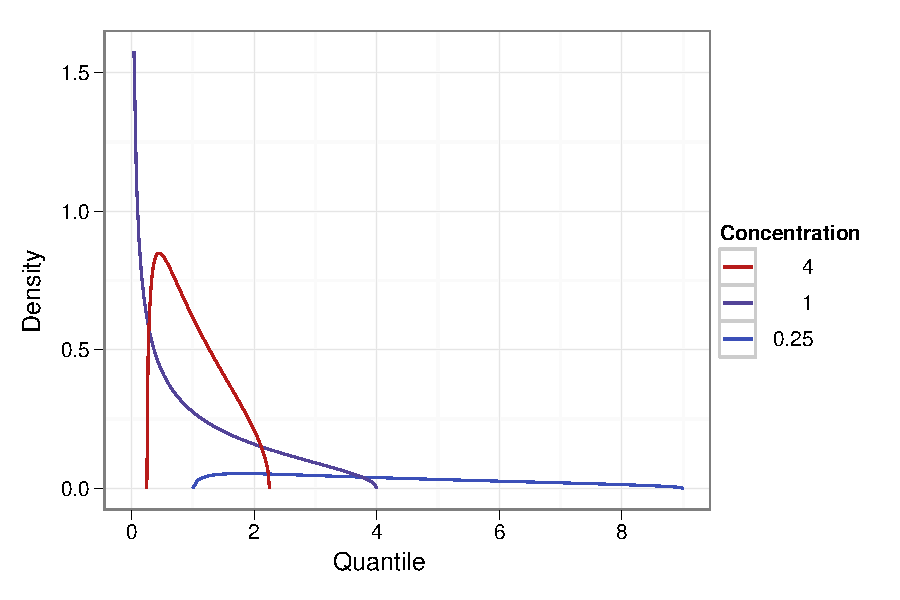
\includegraphics{mp-law}
    \caption{
        \captiontitle{The Mar\v{c}enko-Pastur Law}
        Density, $\fMP_\gamma(x)$, plotted against quantile, $x$,
        for concentration $\gamma = 0.25$, $1$, and $4$.  Concentration
        is equal to the number of samples per dimension. For $\gamma < 1$,
        there is an addition point-mass of size $(1 - \gamma)$ at $x = 0$.
    }\label{F:mp-law}
\end{figure}

